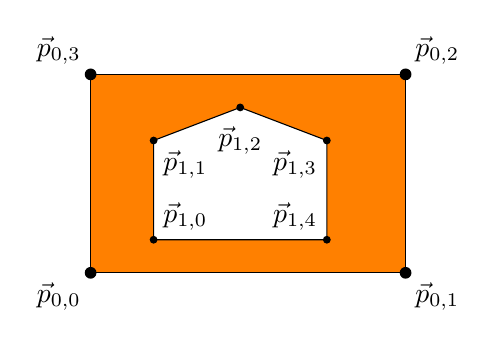
\begin{tikzpicture}[scale=2,yscale=0.7]
  \coordinate (zero) at (0, 0);
  \coordinate (one) at (2.0, 0);
  \coordinate (two) at (2.0, 1.8);
  \coordinate (three) at (0, 1.8);
  \draw[fill=orange]
    (zero) node[below left] {$\vec{p}_{0,0}$}
    -- (one) node[below right] {$\vec{p}_{0,1}$}
    -- (two) node[above right] {$\vec{p}_{0,2}$}
    -- (three) node[above left] {$\vec{p}_{0,3}$}
    -- cycle;
  \foreach \n in {zero,one,two,three}
    \node at (\n)[circle,fill,inner sep=1.5pt]{};

  \coordinate (0) at (0.4, 0.3);
  \coordinate (1) at (1.5, 0.3);
  \coordinate (2) at (1.5, 1.2);
  \coordinate (3) at (0.95, 1.5);
  \coordinate (4) at (0.4, 1.2);
  \draw[fill=white]
    (0) node[above right] {$\vec{p}_{1,0}$}
    -- (1) node[above left] {$\vec{p}_{1,4}$}
    -- (2) node[below left] {$\vec{p}_{1,3}$}
    -- (3) node[below=3.5pt] {$\vec{p}_{1,2}$}
    -- (4) node[below right] {$\vec{p}_{1,1}$}
    -- cycle;
  \foreach \n in {0,1,2,3,4}
    \node at (\n)[circle,fill,inner sep=1pt]{};
\end{tikzpicture}
